\begin{reviewed}

\chapter{Literature Review — \gls{ai} Safety}\label{chap:literature_review}

	\section{\gls{ai} Safety \gls{slr}}\label{ai_safety_slr}

	This \gls{slr} will target the continuous research in the area of \gls{ai} safety by narrowing on a specified search string capable of funneling the amount of peer-reviewed articles from several known Datasets.

	The \gls{slr} wielded research that spanned many fields that would often stray from DevOps or ML Ops pipelines. These including economics and philosophical research, political and corporate regulations and governance systems and numerous high level analysis of the field and current alignment or shallow alignment techniques. Technical research is typically focused on specific issues within well-defined contexts or operational environments, and therefore tends to address problems with shallow alignment\cite{milliere_normative_2025, mcintosh_inadequacy_2024}. Because of this, and since the \gls{ai} field is evolving at a pace that's sometimes hard for peer-reviewed literature to keep up, snowballing was introduced to bring in other relevant articles and gray literature\cite{wohlin_guidelines_2014}. The related table can be found in Appendix \ref{sec:snowballing_articles_slr}.

	With this in mind, a systemic search for literature in all the databases was conducted, applying ever more strict filters to narrow the search to only the most relevant articles. The progress made in this phase can be seen documented on Table \ref{tab:slr1_filters}, the inclusion and exclusion criteria across filters are cleanly defined in Table \ref{tab:inclusion_exclusion_criteria}. 

	\begin{table}[htbp]
		\centering
		\caption{Selection filters to narrow related work for the \gls{slr}}
		\label{tab:slr1_filters}
		\begin{threeparttable}
			\begin{tabular}{lcccccc}
				\toprule
				\textbf{Database} & \textbf{Filter 1}                                                                                                      & \textbf{Filter 2}                                                                                                     & \textbf{Filter 3}                                                                                                     & \textbf{Filter 4} & \textbf{Filter 5} & \textbf{Snowballing} \\
				\midrule
				Scopus            & \href{https://www.scopus.com/results/results.uri?sort=plf-f                                                            & src=s                                                                                                                 & sl=289                                                                                                                & s=(+                                                         %22artificial+intelligence%22+OR+%22LLM*%22+OR+%22generative+AI%22+OR+%22gen+AI%22+OR+%22large+language+model*%22+OR+%22AGI%22+OR+%22Artificial+General+Intelligence%22)+AND+(+%22AI+safety%22+)+AND+NOT+(+%22robot*%22+OR+%22industrial%22+OR+%22manufacturing%22+OR+%22user+experience%22+OR+%22UX%22+OR+%22clinical%22+OR+%22healthcare%22+OR+%22medical%22+)&origin=searchadvanced&limit=10}{1,239} & \href{https://www.scopus.com/results/results.uri?sort=cp-f&src=s&sot=a&sdt=a&sl=297&s=TITLE-ABS%28%28%22artificial+intelligence%22+OR+%22LLM*%22+OR+%22generative+AI%22+OR+%22gen+AI%22+OR+%22large+language+model*%22+OR+%22AGI%22+OR+%22Artificial+General+Intelligence%22%29+AND+%28+%22AI+safety%22%29+AND+NOT+%28%22robot*%22+OR+%22industrial%22+OR+%22manufacturing%22+OR+%22user+experience%22+OR+%22UX%22+OR+%22clinical%22+OR+%22healthcare%22+OR+%22medical%22%29%29&origin=searchadvanced&limit=200}{167} & \href{https://www.scopus.com/results/results.uri?sort=plf-f&src=s&sot=a&sdt=a&cluster=scosubtype%2C%22ar%22%2Ct%2C%22re%22%2Ct%2Bscolang%2C%22English%22%2Ct&sl=340&s=TITLE-ABS%28%28%22artificial+intelligence%22+OR+%22LLM*%22+OR+%22generative+AI%22+OR+%22gen+AI%22+OR+%22large+language+model*%22+OR+%22AGI%22+OR+%22Artificial+General+Intelligence%22%29+AND+%28+%22AI+safety%22%29+AND+NOT+%28%22robot*%22+OR+%22industrial%22+OR+%22manufacturing%22+OR+%22user+experience%22+OR+%22UX%22+OR+%22clinical%22+OR+%22healthcare%22+OR+%22medical%22%29%29+AND+PUBYEAR+%3E+2024+AND+PUBYEAR+%3C+2027&origin=searchadvanced&limit=10}{24} & 16 & 16 & \multirow{7}{*}{\centering +15\textsuperscript{*}} \\
				\cmidrule(lr){1-6}
				Web Of Science    & \href{https://www.webofscience.com/wos/woscc/summary/3ef8a031-9a23-493a-a8a1-7c3119363059-0184fac295/relevance/1}{260} & \href{https://www.webofscience.com/wos/woscc/summary/0468ac8e-28ef-4911-b65b-b5c9c4fb1f59-0184fac96b/relevance/1}{79} & \href{https://www.webofscience.com/wos/woscc/summary/9c4a7bda-e4bf-49f1-afb3-59e496719940-0184faf651/relevance/1}{29} & 20                & 17                &                      \\
				\cmidrule(lr){1-6}
				IEEE              & \href{https://ieeexplore.ieee.org/search/searchresult.jsp?action=search                                                & newsearch=true                                                                                                        & matchBoolean=true                                                                                                     & queryText=(                                                  %22All%20Metadata%22:%22artificial%20intelligence%22%20OR%20%22All%20Metadata%22:%22LLM*%22%20OR%20%22All%20Metadata%22:%22generative%20AI%22%20OR%20%22All%20Metadata%22:%22gen%20AI%22%20OR%20%22All%20Metadata%22:%22large%20language%20model*%22%20OR%20%22All%20Metadata%22:%22AGI%22%20OR%20%22All%20Metadata%22:%22Artificial%20General%20Intelligence%22)%20AND%20(%22All%20Metadata%22:%22AI%20safety%22)%20NOT%20(%22All%20Metadata%22:%22robot*%22%20OR%20%22All%20Metadata%22:%22industrial%22%20OR%20%22All%20Metadata%22:%22manufacturing%22%20OR%20%22All%20Metadata%22:%22user%20experience%22%20OR%20%22All%20Metadata%22:%22UX%22%20OR%20%22All%20Metadata%22:%22clinical%22%20OR%20%22All%20Metadata%22:%22healthcare%22%20OR%20%22All%20Metadata%22:%22medical%22)}{95} & \href{https://ieeexplore.ieee.org/search/searchresult.jsp?action=search&newsearch=true&matchBoolean=true&queryText=(%22Abstract%22:%22artificial%20intelligence%22%20OR%20%22Abstract%22:%22LLM*%22%20OR%20%22Abstract%22:%22generative%20AI%22%20OR%20%22Abstract%22:%22gen%20AI%22%20OR%20%22Abstract%22:%22large%20language%20model*%22%20OR%20%22Abstract%22:%22AGI%22%20OR%20%22Abstract%22:%22Artificial%20General%20Intelligence%22)%20AND%20(%22Abstract%22:%22AI%20safety%22)%20NOT%20(%22Abstract%22:%22robot*%22%20OR%20%22Abstract%22:%22industrial%22%20OR%20%22Abstract%22:%22manufacturing%22%20OR%20%22Abstract%22:%22user%20experience%22%20OR%20%22Abstract%22:%22UX%22%20OR%20%22Abstract%22:%22clinical%22%20OR%20%22Abstract%22:%22healthcare%22%20OR%20%22Abstract%22:%22medical%22)}{35} & \href{https://ieeexplore.ieee.org/search/searchresult.jsp?action=search&matchBoolean=true&queryText=(%22All%20Metadata%22:%22artificial%20intelligence%22%20OR%20%22All%20Metadata%22:%22LLM*%22%20OR%20%22All%20Metadata%22:%22generative%20AI%22%20OR%20%22All%20Metadata%22:%22gen%20AI%22%20OR%20%22All%20Metadata%22:%22large%20language%20model*%22%20OR%20%22All%20Metadata%22:%22AGI%22%20OR%20%22All%20Metadata%22:%22Artificial%20General%20Intelligence%22)%20AND%20(%22All%20Metadata%22:%22AI%20safety%22)%20NOT%20(%22All%20Metadata%22:%22robot*%22%20OR%20%22All%20Metadata%22:%22industrial%22%20OR%20%22All%20Metadata%22:%22manufacturing%22%20OR%20%22All%20Metadata%22:%22user%20experience%22%20OR%20%22All%20Metadata%22:%22UX%22%20OR%20%22All%20Metadata%22:%22clinical%22%20OR%20%22All%20Metadata%22:%22healthcare%22%20OR%20%22All%20Metadata%22:%22medical%22)&highlight=true&matchPubs=true&refinements=ContentType:Journals&ranges=2024_2025_Year&returnFacets=ALL}{14} & 11 & 7 & \\
				\cmidrule(lr){1-6}
				ACM               & \href{https://dl.acm.org/action/doSearch?fillQuickSearch=false                                                         & target=advanced                                                                                                       & expand=dl                                                                                                             & field1=AllField   & text1=                                   %28%22artificial+intelligence%22+OR+%22LLM*%22+OR+%22generative+AI%22+OR+%22gen+AI%22+OR+%22large+language+model*%22+OR+%22AGI%22+OR+%22Artificial+General+Intelligence%22%29+AND+%28+%22AI+safety%22%29+AND+NOT+%28%22robot*%22+OR+%22industrial%22+OR+%22manufacturing%22+OR+%22user+experience%22+OR+%22UX%22+OR+%22clinical%22+OR+%22healthcare%22+OR+%22medical%22%29}{114} & \href{https://dl.acm.org/action/doSearch?fillQuickSearch=false&target=advanced&expand=dl&AllField=Abstract%3A%28%28%22artificial+intelligence%22+OR+%22LLM*%22+OR+%22generative+AI%22+OR+%22gen+AI%22+OR+%22large+language+model*%22+OR+%22AGI%22+OR+%22Artificial+General+Intelligence%22%29+AND+%28+%22AI+safety%22%29+AND+NOT+%28%22robot*%22+OR+%22industrial%22+OR+%22manufacturing%22+OR+%22user+experience%22+OR+%22UX%22+OR+%22clinical%22+OR+%22healthcare%22+OR+%22medical%22%29%29}{11} & \href{https://dl.acm.org/action/doSearch?fillQuickSearch=false&target=advanced&expand=dl&AfterMonth=1&AfterYear=2024&BeforeMonth=12&BeforeYear=2025&AllField=Abstract%3A%28%28%22artificial+intelligence%22+OR+%22LLM*%22+OR+%22generative+AI%22+OR+%22gen+AI%22+OR+%22large+language+model*%22+OR+%22AGI%22+OR+%22Artificial+General+Intelligence%22%29+AND+%28+%22AI+safety%22%29+AND+NOT+%28%22robot*%22+OR+%22industrial%22+OR+%22manufacturing%22+OR+%22user+experience%22+OR+%22UX%22+OR+%22clinical%22+OR+%22healthcare%22+OR+%22medical%22%29%29}{8} & 8 & 5 & \\
				\cmidrule(lr){1-6}
				EBSCO             & \href{https://research.ebsco.com/c/2i6b6x/search/results?q=                                                                                                                                                                                                                                                                                                                                                                           %28%22artificial+intelligence%22+OR+%22LLM*%22+OR+%22generative+AI%22+OR+%22gen+AI%22+OR+%22large+language+model*%22+OR+%22AGI%22+OR+%22Artificial+General+Intelligence%22%29+AND+%22AI+safety%22+NOT+%28%22robot*%22+OR+%22industrial%22+OR+%22manufacturing%22+OR+%22user+experience%22+OR+%22UX%22+OR+%22clinical%22+OR+%22healthcare%22+OR+%22medical%22%29&autocorrect=y&limiters=None&searchMode=all&searchSegment=all-results&sqId=sq%3A97428daf-a9be-49ad-b6b5-a79fb60a0088}{4,709} & \href{https://research.ebsco.com/c/2i6b6x/search/results?q=AB%20(%22artificial%20intelligence%22%20OR%20%22LLM*%22%20OR%20%22generative%20AI%22%20OR%20%22gen%20AI%22%20OR%20%22large%20language%20model*%22%20OR%20%22AGI%22%20OR%20%22Artificial%20General%20Intelligence%22)%20AND%20AB%20(%22AI%20safety%22)%20NOT%20AB%20(%22robot*%22%20OR%20%22industrial%22%20OR%20%22manufacturing%22%20OR%20%22user%20experience%22%20OR%20%22UX%22%20OR%20%22clinical%22%20OR%20%22healthcare%22%20OR%20%22medical%22)&autocorrect=y&limiters=None&searchMode=all&searchSegment=all-results&skipResultsFetch=true&sqId=sq%3A0590f29e-b56b-4417-8760-50637ae6292a}{2,949} & \href{https://research.ebsco.com/c/2i6b6x/search/results?q=AB+%28%22artificial+intelligence%22+OR+%22LLM*%22+OR+%22generative+AI%22+OR+%22gen+AI%22+OR+%22large+language+model*%22+OR+%22AGI%22+OR+%22Artificial+General+Intelligence%22%29+AND+AB+%28%22AI+safety%22%29+NOT+AB+%28%22robot*%22+OR+%22industrial%22+OR+%22manufacturing%22+OR+%22user+experience%22+OR+%22UX%22+OR+%22clinical%22+OR+%22healthcare%22+OR+%22medical%22%29&autocorrect=y&facetFilter=sourceTypes%3AMTYwTU4%3D%2CLanguage%3AZW5nbGlzaA%3D%3D&limiters=DT1%3A2024-01-01%2F2026-01-01%2CRV%3AY%2CFT%3AY&searchMode=all&searchSegment=all-results&skipResultsFetch=true&sqId=sq%3Ad1d6e143-5e1a-4724-ba27-6bb8ca0cee39}{50} & 24 & 18 & \\
				\midrule
				\textbf{Total}    & 6668                                                                                                                   & 3241                                                                                                                  & 125                                                                                                                   & 79                & 63                & 78                   \\
				\bottomrule
			\end{tabular}
			\begin{tablenotes}
				\small
				\item[*] The Alignment Research Center is counted as one entry, though the non-profit research organization has published multiple works.
				\item Filter 1 = All fields, All documents
				\item Filter 2 = Abstract, All documents
				\item Filter 3 = Peer-reviewed \& other inclusion/exclusion criteria
				\item Filter 4 = Remove duplicates (duplicate items were kept in the DBs with fewer entries)
				\item Filter 5 = After Abstracts Screened and Concept Matrix
				\item Snowballing = Full-text Document Assess
			\end{tablenotes}
		\end{threeparttable}
	\end{table}

	\begin{table}[htbp]
		\centering
		\caption{Inclusion and exclusion criteria applied}
		\label{tab:inclusion_exclusion_criteria}
		\begin{tabular}{c c}
			\toprule
			\textbf{Inclusion Criteria} & \textbf{Exclusion Criteria}                \\
			\midrule
			Matched by Search String    & Advertisement, Keynote, or Job Post        \\
			Published in and after 2024 & No publication date                        \\
			Peer-Reviewed               & No match in \gls{cm}             \\
			Written in English          & Only one match in \gls{cm} and divergent subject \\
			Full-text accessible        &                                            \\
			\bottomrule
		\end{tabular}
	\end{table}

A noteworthy consideration is the growth that the \gls{ai} safety field has experienced in the past couple of years. Since the advent of \glspl{llm} that \gls{ai} has been a booming topic, this can be verified in the volume of publications like can be seen in Figure \ref{fig:all-ai-timegraph}, \begin{toreview} or in the volume of web searches like shown in Figure \ref{fig:google_trends_ai_safety}. \end{toreview}

\begin{figure}[htbp]
	\centering
	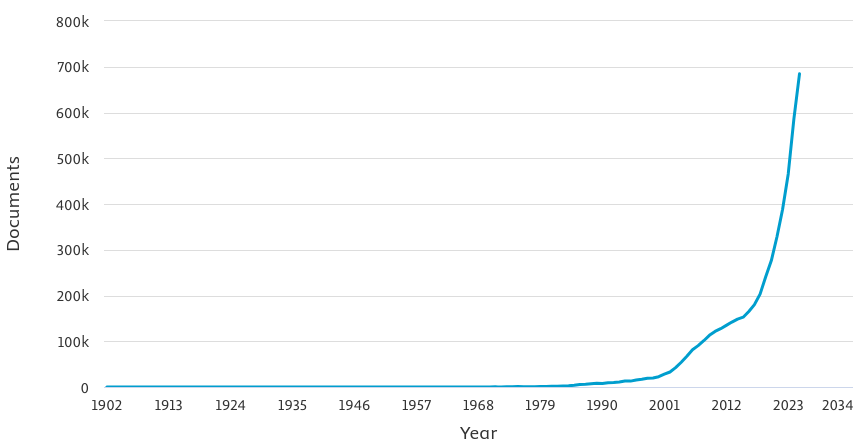
\includegraphics[width=0.75\textwidth]{./src/imgs/All_AI_timeGraph_Scopus}
	\caption{Number of documents mentioning \gls{ai} (Scopus). At the end of 2025 there were 684527 documents.}
	\label{fig:all-ai-timegraph}
\end{figure}

\begin{figure}[htbp]
	\centering
	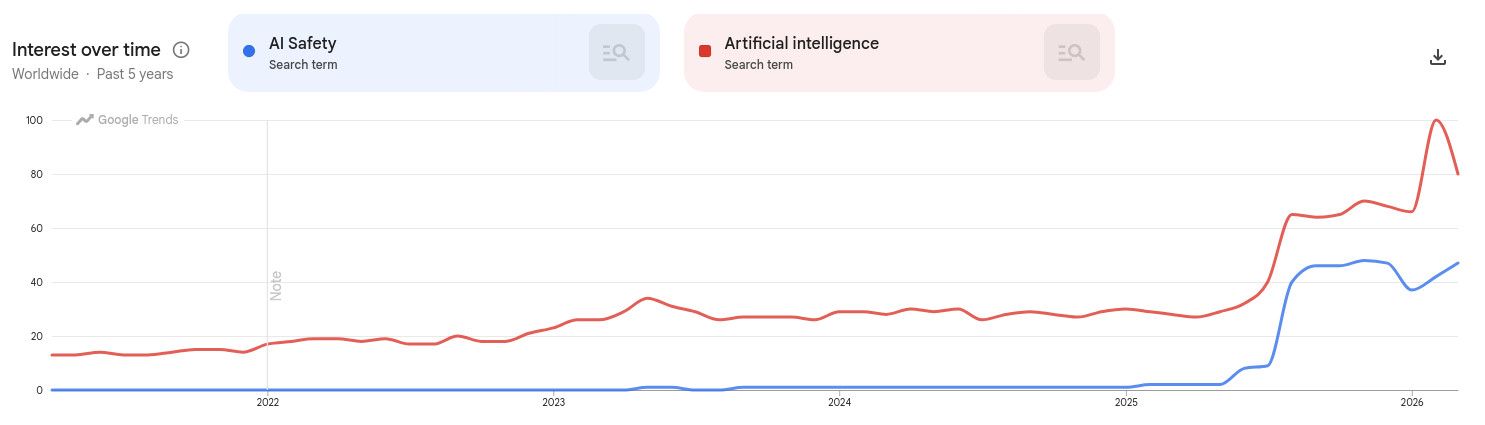
\includegraphics[width=0.75\textwidth]{./src/imgs/GoogleTrendsAI_Safety.jpg}
	\caption{Volume of Web Searches of the terms ``AI Safety'' and ``Artificial Intelligence''}
	\label{fig:google_trends_ai_safety}
\end{figure}

In much the same way, \gls{ai} safety publications have also enjoyed an increase in output, this can be verified in the Scopus database as seen in Figure \ref{fig:ai-safety-timegraph}, especially with the release of ChatGPT on November 30, 2022. Albeit with fewer advancements, largely due to financial incentives \cite{eto_state_global_ai_research_2024, ahmed_narrow_depth_breadth_corporate_2024, hemphill_advanced_2025}. \begin{toreview} The same can be verified in general web searches, Figure \ref{fig:google_trends_ai_safety}. \end{toreview}

\begin{figure}[htbp]
	\centering
	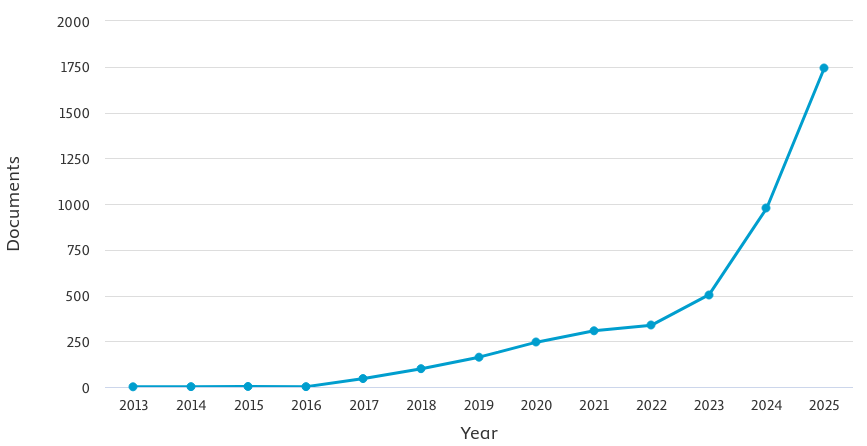
\includegraphics[width=0.75\textwidth]{./src/imgs/AI_Safety_timeGraph_Scopus}
	\caption{Number of documents mentioning \gls{ai} (Scopus) and containing "\gls{ai} safety". At the end of 2025 there were 1742 documents.}
	\label{fig:ai-safety-timegraph}
\end{figure}

\end{reviewed}